\section{Forundersøgelse}\label{ch:forundersoegelse}

\begin{center}
\begin{tabular}{ |p{100pt}|p{100pt}|p{100pt}| }
    \hline
    Medarbjeder & Opgave & Mål \\
    \hline\hline
    Sælgere
    & udføre salg & salget er udført \\
    \hline
    & køre forberelse & sælger er klar til at køre \\
    \hline
    Lagermedarbejder
    & påfyld bil & bil er fuld \\
    \hline
    & modtag ny levering & levering er i kølerbokse \\
    \hline
    Depotchef
    & registrer salg of dagsomstætning på biller & aktiviter fra dagen før er bogført \\
    \hline
    & udprinte odrer & orderer er klar til sælgere \\
    \hline
    & lave router & router er klar til sælgerer \\
    \hline
    & bestemmer lager orden & lageret passer markets efterspørgsel \\
    \hline
\end{tabular}
\end{center}

\begin{center}
\begin{tabular}{ |p{90pt}|p{90pt}|p{90pt}|p{90pt}| }
    \hline
    Medarbjeder & Opgave & Mål & Trin \\
    \hline\hline
    Ismand
    & Modtager ny ordre & Ordren er registreret som værende solgt. &
    - modtag ordre fra kunde \\
    &&&
    - Ordren med tilhørende adresse  registreres \\
    &&&
    - Adressen på ordren printes ud og lægges i den rigtige kasse til næste dag \\
    &&&
    - Den udprintede ordre tages med i bilen \\
    &&&
    - Ordren leveres til kunden på turen \\
    &&&
    - Kunden underskriver ordren \\
    &&&
    - Den underskrevene ordre afleveres til chefen \\
    \hline
    Ismand & Annuler ordre & Ordren er annulleret &
    - Modtag ordre fra kunde \\
    &&&
    - under “registrer ordre”, før samtlige trin er gennemført, kontakter kunden depotet og vil have ordre annulleret \\
    &&&
    - Ordren annulleres. \\
    \hline
    Lagermedarbejder
    & Isbilen skal ryddes op & Isbilens bokse er ryttet op så der er plads til nye varern &
    - Ismanden åbner en boks med is \\
    &&&
    - Ismanden omrokerer pakkerne således at der er bedre plads til nye pakker næste dag \\
    &&&
    - Ismanden lukker boksen \\
    &&&
    - Gentages indtil alle bokse er ryddet op. \\
    \hline
    Lagermedarbejder
    & Modtager nye varer & Varerne er registreret og lagt i fryseren &
    - Nye varer ankommer til depotet \\
    &&&
    - Varerne læsses af på paller \\
    &&&
    - Varerne registreres og godkendes så mængden stemmer \\
    &&&
    - Varerne lægges ind i fryseren \\
    \hline
    Lagermedarbejder & Varer skal afskrives & Varer er afskrevet &
    - Lageret er blevet talt op \\
    &&&
    - Under optælling er der fundet varer som er udløbet \\
    &&&
    - Varerne tilsidesættes \\
    &&&
    - Varerne registreres som udløbet i systemet \\
    &&&
    - Varerne er afskrevet og kan ikke sælges \\
    \hline
    Depotchef
    & registrer salg of dagsomstætning på biller & aktiviter fra dagen før er bogført &
    - test1 \\
    &&&
    - test2 \\
    \hline
    & udprinte odrer & orderer er klar til sælgere &
    - test1 \\
    &&&
    - test2 \\
    \hline
    & lave router & router er klar til sælgerer &
    - test1 \\
    &&&
    - test2 \\
    \hline
    & bestemmer lager orden & lageret passer markets efterspørgsel &
    - test1 \\
    &&&
    - test2 \\
    \hline
\end{tabular}
\end{center}

\begin{figure}[H]
    \centering
    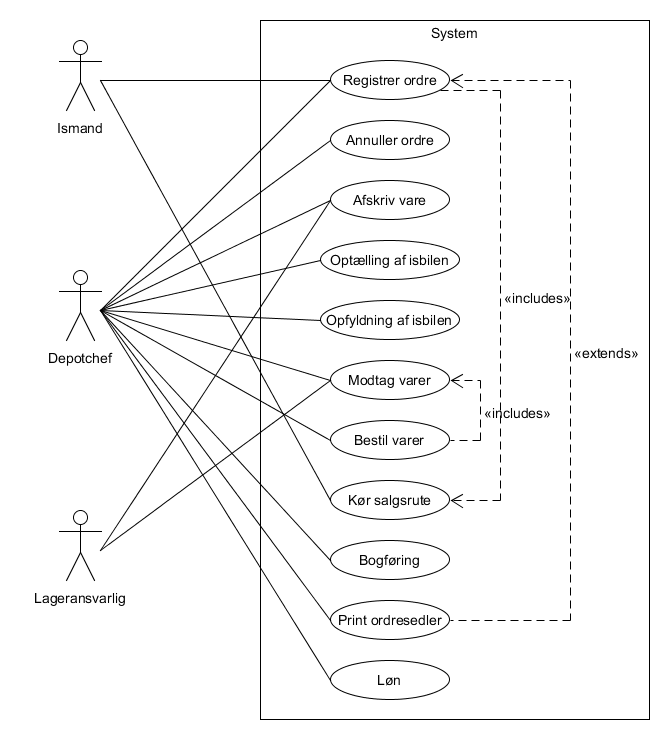
\includegraphics[width=\textwidth]{figures/Forundersøgelse/use_case_diagram.png}
    \caption{Use case diagram}
    \label{fig:use_case_diagram}
\end{figure}

\begin{figure}[H]
    \centering
    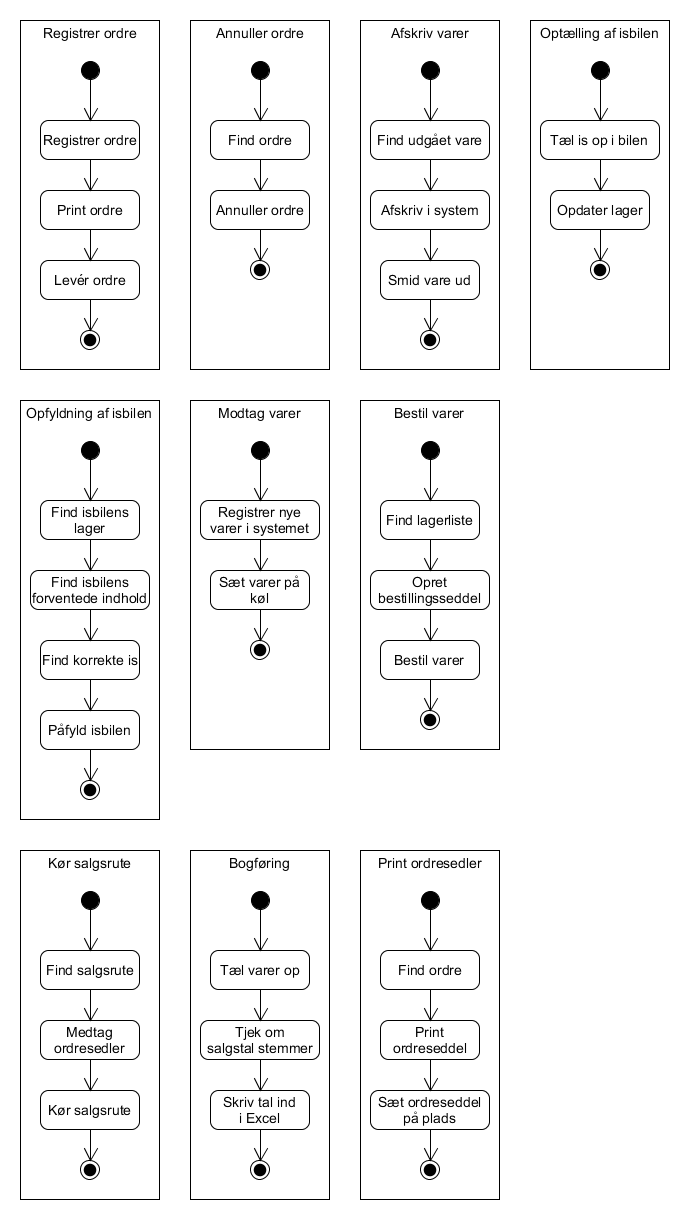
\includegraphics[width=\textwidth]{figures/Forundersøgelse/workflows.png}
    \caption{Workflow diagram}
    \label{fig:workflows}
\end{figure}